\section{Question 3: Text Summarization}

\subsection{Dataset Description}

Question 3 compares extractive and abstractive summarization on CNN/DailyMail \cite{see2017get}, a news summarization benchmark pairing long-form news articles with short highlight summaries written by editors. The completed comparison uses a 10{,}000-example training slice together with matched 50-example validation and 50-example test evaluation slices so that both models are scored on exactly the same articles under the same export contract. The emphasis is therefore a controlled head-to-head comparison of summary quality rather than benchmark-scale saturation.

Even with that limitation, CNN/DailyMail remains an appropriate benchmark for this comparison because the articles are substantially longer than the references and require both content selection and compression. This makes the task a natural contrast between a sentence-ranking baseline such as TextRank and a pretrained abstractive model that can rewrite source content into shorter, reference-style summaries.

\subsection{Preprocessing and Method}

The Q3 pipeline performs shared article cleanup, truncates long inputs to 900 words, and evaluates all models with the same lexical metrics. The extractive baseline is a TF-IDF based TextRank summarizer \cite{mihalcea2004textrank}: sentences are treated as graph nodes, pairwise cosine similarities define weighted edges, and PageRank scores determine which three sentences are selected for the final summary. The configuration uses damping 0.85 and allows up to 40 candidate sentences per article.

The abstractive baseline uses the pretrained \nolinkurl{sshleifer/distilbart-cnn-12-6} checkpoint from the DistilBART family. It is derived from BART-style sequence-to-sequence pretraining \cite{lewis2020bart} and is used here without additional fine-tuning. Inputs are tokenized up to 1024 tokens, decoding uses beam search with 4 beams, and generated summaries are constrained between 56 and 142 tokens with length penalty 2.0 and no-repeat 3-gram blocking. This design keeps the comparison practical while still testing the main assignment question: whether an abstractive model can produce more reference-like summaries than a purely extractive sentence selector.

\subsection{Results}

Table~\ref{tab:q3_overall_results} summarizes the matched two-model comparison. On the test split, DistilBART reaches ROUGE-1 0.4204, ROUGE-2 0.1865, ROUGE-L 0.2785, BLEU 0.1234, METEOR 0.4123, and BERTScore 0.8831. TextRank reaches 0.3301, 0.1170, 0.2194, 0.0696, 0.3233, and 0.8677 respectively. The abstractive model outperforms TextRank on every metric on both validation and test.

\begin{table}[H]
\centering
\small
\setlength{\tabcolsep}{4pt}
\begin{tabularx}{\linewidth}{>{\raggedright\arraybackslash}l >{\raggedright\arraybackslash}l c c c c c c}
\toprule
Model & Split & ROUGE-1 & ROUGE-2 & ROUGE-L & BLEU & METEOR & BERTScore \\
\midrule
TextRank   & Validation & 0.3522 & 0.1458 & 0.2316 & 0.0982 & 0.3422 & 0.8679 \\
TextRank   & Test       & 0.3301 & 0.1170 & 0.2194 & 0.0696 & 0.3233 & 0.8677 \\
DistilBART & Validation & \textbf{0.4468} & \textbf{0.2235} & \textbf{0.3189} & \textbf{0.1831} & \textbf{0.4145} & \textbf{0.8858} \\
DistilBART & Test       & \textbf{0.4204} & \textbf{0.1865} & \textbf{0.2785} & \textbf{0.1234} & \textbf{0.4123} & \textbf{0.8831} \\
\bottomrule
\end{tabularx}
\caption{Controlled Q3 comparison on the exported 50-example validation and 50-example test evaluation slices. DistilBART outperforms TextRank on every metric on both splits.}
\label{tab:q3_overall_results}
\end{table}

Figure~\ref{fig:q3_test_metric_comparison} visualizes the same test-set ranking. DistilBART leads TextRank on every exported metric, with especially clear gaps on METEOR, ROUGE-1, and ROUGE-2.

\begin{figure}[H]
	\centering
	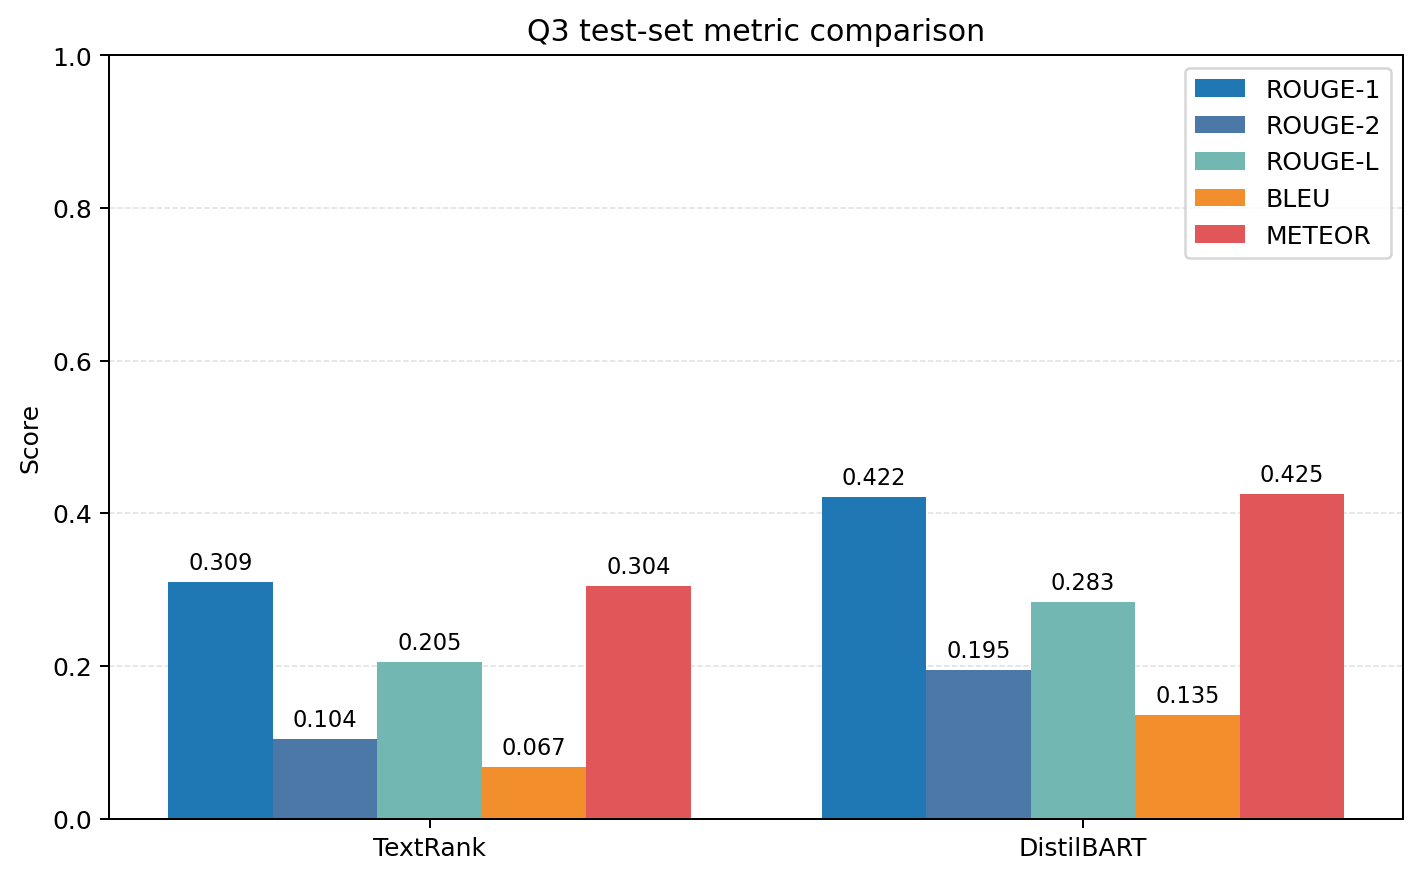
\includegraphics[width=0.92\textwidth]{figures/q3/test_metric_comparison.png}
	\caption{Q3 test-set metric comparison for TextRank and DistilBART.}
	\label{fig:q3_test_metric_comparison}
\end{figure}

The largest absolute test improvements are in METEOR (+0.0890), ROUGE-1 (+0.0903), and ROUGE-2 (+0.0695). BERTScore also favors DistilBART (0.8831 vs.\ 0.8677), confirming that the abstractive model produces semantically closer summaries even when the n-gram overlap gap is modest. Because the evaluation slice is intentionally controlled and identical across both systems, the most important point is the consistency of the model ranking across all six metrics rather than the absolute size of the scores alone.

\subsection{Qualitative Analysis}

The qualitative examples mirror the aggregate scores. In the teen-driver distraction article from the validation split, DistilBART produces a compact summary that preserves the central finding that distraction contributes to nearly 60\% of serious teen crashes and correctly identifies passengers and cellphones as the main sources. The corresponding TextRank output is longer, more repetitive, and much less reference-like. A second validation example on Aaron Cook's Moldovan citizenship decision shows the same pattern: both models remain on topic, but the abstractive summary keeps the citizenship, Rio 2016, and Team GB exclusion details while dropping more of the surrounding narrative.

The test split also shows that the abstractive model is not uniformly strong. In the Syrian refugee first-person article, DistilBART stays broadly on topic but still misses key reference details such as the speaker's identity and the specific 12-day journey framing. That limitation matters because it shows that better lexical overlap does not automatically guarantee perfect factual focus. Even so, across the inspected examples DistilBART is generally more concise and closer to the structure of the human-written highlights, whereas TextRank often copies lead sentences or redundant clauses directly from the article.

\subsection{Discussion}

The Q3 results support a clear conclusion: on this task, the pretrained abstractive baseline is stronger than the extractive TextRank baseline under the same reported evaluation protocol. TextRank remains useful as a cheap and interpretable baseline, and it can preserve source facts when important content is already concentrated in the lead sentences. However, it is weaker at compression and at matching the short editor-style summaries used as references in CNN/DailyMail.

Within the reported setup, the section provides a complete metric picture across ROUGE, BLEU, METEOR, and BERTScore, and the best-performing Q3 system is the pretrained DistilBART model rather than TextRank.